\begin{center}
\begin{tikzpicture}[shorten >=1pt,draw=black!50, x = 1 cm, y = 1cm,  node distance=20pt]
%\draw[draw=black, use as bounding box](-10,12) rectangle (10,0);
\draw[use as bounding box, anchor = north west,draw,dashed,gray] (-5.65,-3.25) rectangle (5.65,3.25);
\clip (-5.7,-3.3) rectangle (5.7,3.6);
\node[anchor=north west,text badly centered, text width=10 cm] at (-5.5,3.2) {The richness of the representation also affects learning rate:};

\visible<2->{\node  (liex) at (0,0) {{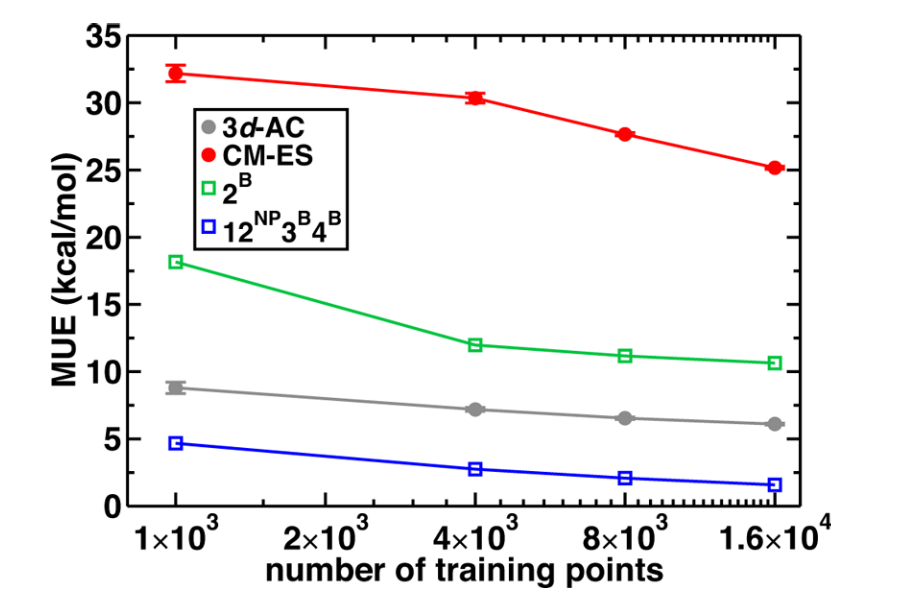
\includegraphics[width=7.5 cm]{representations/figures/learn_rate}}};}


\end{tikzpicture}
\end{center}

